\section{Design}\label{sec:method}

\lancet is a dynamic symbolic execution tool that aims to generate {\em scaling inputs} for programs: inputs that cause programs to run for a long time. In contrast to black-box stress-generation tests, \lancet targets particular loops for scaling. It attempts to generate inputs that will cause a chosen loop to execute a specified (large) number of iterations. In this way, particular regions of code can be targeted to see how they behave under heavy load. This section first describes \lancet's behavior at a high level, and then explains \lancet's various components in more detail. %For ease of exposition, this section assumes that there is just one symbolic input parameter in the program under test,\footnote{Note that other variables dependent on this input parameter may also be symbolic} and that parameter is numeric ({\em e.g.}, a single integer parameter). Section~\ref{sec:extensions} discusses how \lancet deals with more general inputs.
For ease of exposition, this section assumes that the program under test takes a single symbolic string as input.
%Section~\ref{sec:extensions} discusses how \lancet deals with more general inputs.

\subsection{Overview of \lancet}
\label{sec:overview}

\lancet has two modes of operation: {\em explicit} mode, which uses traditional dynamic symbolic execution techniques to generate inputs that run a target loop for a specified, small number of iterations, and {\em inference} mode, which uses statistical techniques to generate inputs that run a target loop for a large number of iterations. These modes are described in more detail in Sections~\ref{sec:explicit-mode} and~\ref{sec:inference-mode}, respectively. At a high level, they behave as described next.

\lancet's explicit mode begins by using programmer annotations to identify the target loops (Section~\ref{sec:target-loop}). For each target loop, \lancet then generates a path condition that satisfy a {\em loop-iteration meta-constraint} that the target loop executes exactly $N$ times. For small $N$, this is done by a custom {\em loop-centric} path-exploration heuristic (Section~\ref{sec:loop-centric}).

While the explicit mode suffice to generate path constraints that run a loop a small number of times, it is impractical for large $N$: \eg running a loop a thousand times will require two orders of magnitude more invocations to \lancet's constraint solver than running a loop ten times, and will be unacceptably slow. \lancet's novel approach to this problem is to determine the path constraints that satisfy the loop-iteration meta-constraint for a large $N$ {\em without performing symbolic execution}.

\begin{figure}[tbp]
  \centering
  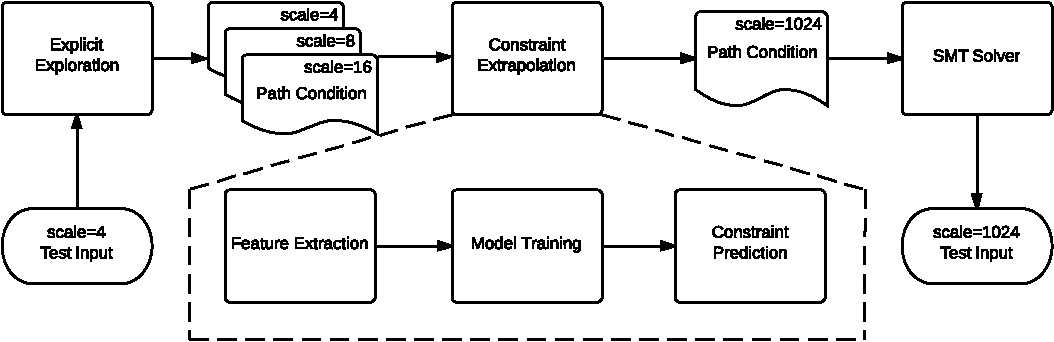
\includegraphics[width=\linewidth]{figures/lancet} %TODO need to update
  \caption{High level flow of \lancet's inference-mode approach for generating inputs for a given loop.}
  \label{fig:method}
\end{figure}

% \lancet's inference mode operates as shown in Figure~\ref{fig:method}. First, \lancet uses its explicit mode to generate {\em multiple} path constraint sets, each for different small values of $N$. It then analyzes those path constraints to separate the constraints in those sets into {\em validity constraints}---constraints that ensure that inputs are well-formed---and {\em scaling constraints}---constraints that determine how many times the target loop runs (Section~\ref{sec:validity-constraints}). \lancet then uses the scaling constraints to train a statistical model that relates the value of $N$ to the associated scaling constraints, and uses this model to {\em predict what the scaling constraints would look like} for large $N$ (Section~\ref{sec:constraint-inference}). These predicted scaling constraints are then perturbed slightly to account for modeling error and combined with the validity constraints to produce a new constraint set, which can be solved with a constraint solver, generating a large-scale input for the program (Section~\ref{sec:input-generation}). 

\lancet's inference mode operates as shown in Figure~\ref{fig:method}.
First, \lancet uses its explicit mode to generate {\em multiple} path conditions, for a pair of consecutive numbers of iterations $M$ and $M+1$, using a symbolic input string of $L$ bytes.\footnote{Multiple path conditions may result in the same number of iterations.}
It then looks into pairs of path conditions for different numbers of iterations and identifies the {\em incremental set}, the set of path constraints that {\em only} exist in the $M+1$-iteration path conditions.
\lancet then extrapolates the path condition of $N$ iterations by appending $N-M$ copies of the incremental set to the $M$-iteration path condition, each projected to appropriate offsets beyond the initial $L$ bytes of the input string using a linear regression model (Section~\ref{sec:constraint-inference}).
Finally, the predicted $N$-iteration path condition is solved with a constraint solver to generate a large-scale input for the program (Section~\ref{sec:input-generation}), which is then verified in real execution of the program. Depending on the result of verification, \lancet may restart the explicit mode to generate more training data and refine the large-scale input based on new path conditions discovered in the explicit mode.

% TODO Move the following to detail sections
% Inference is done on differential constraints produced by the same branch instruction.
% All differential constraints are grouped by the branch instructions that introduce them.
% Though always being introduced by the same instruction, the terms in a constraint may change from iteration to iteration. 
% \lancet applies a separate model to predict the value of each term, concrete or symbolic, for each of the additional $N-M$ iterations.
% If every iteration took the same path through the loop body, the same set of branches, thereby the same path condition would appear again and again.
% Given the number of times each differential constraint appears in a single iteration, \lancet then projects the number of times it would appear should the loop run for $N$ iterations ($N \gg M$).
% Finally, if a different path were taken in an iteration after the first $M$ iterations, the predicted path condition would miss some constraints from the new path, generating inputs that would not be able to reach $N$ iterations or failing to generate any inputs at all because of contradictory constraints.
% In this case, \lancet retreats to the explicit mode to discover more distinct paths through the loop body before going into the inference mode again.

Crucially, once the initial training phase of \lancet is complete, inputs that target {\em any scale} can be generated at the same overhead (though potentially different levels of accuracy), making \lancet a truly scalable approach to generating large-scale, stress-test inputs.

\paragraph{Running example}

% To aid in the discussion of the components and operation of \lancet, we will use a running example of matrix-vector multiply, as shown in Figure~\ref{fig:example}. A few salient points: (i) the code computes $y = A*x$, where $A$ is an $u \times v$ matrix, and $x$ is a $v \times 1$ vector; (ii) though there are two input variables to this code, $u$ is fixed at 10, to satisfy the single-variable constraint mentioned above; (iii) though the size of the matrix and the size of the vector are independent inputs, they are required to be equal to each other, leading to a single degree of freedom in scaling (see Section~\ref{sec:multivar} for more discussion); (iv) though the program generates matrix and vector values, the control flow of the program is independent of those values (see Section~\ref{sec:structured} for how \lancet handles value-dependent control flow).
%
% \begin{figure}[tb]
% \centering
% \begin{lstlisting}
% int u = 10; //input variable, fixed to 10 (* \label{line:u} *)
% int v1 = /* read */; //symbolic, columns in matrix
% int v2 = /* read */; //symbolic, rows in vector

% if (v1 != v2) exit(1); //dimensions match (* \label{line:v1neqv2} *)
% if (v1 <= 0) exit(1); //vector not zero (* \label{line:v1le0} *)

% float A[u][v1] = /* generate random matrix */
% float x[v2] = /* generate random vector */
% float y[v2] = /* initialize vector to zero */

% [[loop_target]] (* \label{line:annotation} *)
% for (int i = 0; i < v1; i++) { (* \label{line:targetloop} *)
  % for (int j = 0; j < u; j++) { (* \label{line:innerloop} *)
    % y[j] += A[j][i] * x[i];
  % }
% }
% \end{lstlisting}
% \vspace{-5pt}
% \caption{Running example: matrix-vector multiply.}
% \label{fig:example}
% \end{figure}

To aid in the discussion of the components and operation of \lancet, we will use a running example of request parsing from Memcached~\cite{memcached}. A few salient points:
(i) the code parses the request string that contains a {\em get} command followed by a list of keys separated by one or more spaces;
(ii) the first function {\tt tokenize\_command} splits the command string (a symbolic string of configurable size received from the Socket layer of \lancet, see Section \ref{sec:socket}) into a list of tokens, stores them as a list of tokens terminated by a length 0 token, then returns the number of tokens retrieved;
%the loop at line~\ref{line:for-loop} scans each byte in the command string, and uses two pointer variables {\tt s} and {\tt e} to pinpoint the start and the end of each token.
(iii) the second function {\tt parse\_get\_command} parses the list of tokens in the target loop (line~\ref{line:while-loop}) and executes the {\em get} command for each key contained in {\tt tokens}.
%Clearly, the number of iterations of the target loop is the same as the number of tokens passed to the function.
(iv) the number of iterations executed by the target loop is determined by the loop in function {\tt tokenize\_command}.
(v) in the following references to this example, we suppose the length of the {\tt command} string is 8 bytes for the ease of exposition.

\begin{figure*}[tbp]
\centering
\begin{lstlisting}
size_t tokenize_command(char *command, token_t *tokens, size_t max_tokens) {
    char *s, *e;
    size_t ntokens = 0;
    size_t len = strlen(command);
    unsigned int i = 0;
    s = e = command;
    for (i = 0; i < len; i++) { @ \label{line:for-loop} @
        if (*e == ' ') { @ \label{line:isspace} @
            if (s != e) { @ \label{line:sneqe} @
                /* add a new token into tokens */
                ntokens++;
                if (ntokens == max_tokens - 1) { e++; s = e; break; }
            }
            s = e + 1;
        }
        e++;
    }
    if (s != e) {
        /* add the last token into tokens */
        ntokens++;
    }
    /* add a terminal token of length 0 into tokens */
    ntokens++;
    return ntokens;
}

void process_get_command(token_t *tokens, size_t ntokens) {
    token_t *key_token = &tokens[KEY_TOKEN]; /* KEY_TOKEN is the offset to the first key */
    [[loop_target]] while(key_token->length != 0) { @ \label{line:while-loop} @
        /* retrieve the key from cache */
        key_token++;
    }
}
\end{lstlisting}
\caption{Running example: request parsing in Memcached.}
\label{fig:example}
\end{figure*}

\subsection{Explicit Mode}
\label{sec:explicit-mode}

The goal of \lancet is to find performance tests that impose a certain load level precisely on a certain part of code in the given program. Specifically, \lancet's test generation is designed for loops and therefore the load level is determined by the trip count of a loop. 

For a given trip count $N$ and a target loop $l$, \lancet's explicit mode uses symbolic execution to generate an execution path that satisfies the meta-constraint that the path executes loop $l$ exactly $N$ times. The symbolic execution engine treats the input as a bitvector of symbolic variables, computes symbolic expressions for input-dependent variables, and accumulates the constraints at every branch to form the set of constraints, \ie the path condition, that must hold when the path is followed in an execution. \lancet obtains a test input for the program that will run $l$ for $N$ iterations by calling an external SMT solver to find concrete values that satisfy the path condition.

\subsubsection{Targeting a loop}
\label{sec:target-loop}

\lancet provides a simple yet powerful interface for user to specify which loops she wants to target using source code annotation. To mark a loop as a target for test generation, the attribute {\tt [[loop\_target]]} needs to be inserted right before the loop statement. In the running example, the loop at line~\ref{line:while-loop} is targeted for test generation.


\subsubsection{Loop-centric search heuristic}
\label{sec:loop-centric}

The powerful multi-path analysis enabled by symbolic execution comes with a price: the path explosion problem. In order to get meaningful results within a reasonable time frame, any symbolic execution tool must steer through the exponentially growing number of paths and prioritize the exploration of the more interesting ones. For example, as demonstrated by KLEE~\cite{klee}, path searching heuristics like random path selection and coverage-optimized search are effective for generating high-coverage tests for complex programs (like {\sc Gnu Coreutils}). However, these heuristics, though good for discovering unexplored code, are ill-suited for the purpose of generating performance tests, because rather than exercising every line of code once, as a functional test suite might, a performance test should instead repeatedly execute critical pieces of code to simulate high loads.

\lancet employs a loop-centric heuristic to guide the search for paths that extend the target loop for a large number of iterations. Following many existing symbolic execution tools, \lancet encapsulates runtime execution information such as program counter, path condition, memory content in a symbolic process. The loop-centric search operates in two modes, the {\em explorer} mode and the {\em roller} mode. 

In explorer mode, \lancet starts the execution with a single symbolic process from program entry, forking a new process at each branch that has a satisfiable path condition (this is the default execution mode for KLEE). If the loop header of the target loop, $l$ is hit by any of these symbolic processes, that process enters roller mode and the other explorer processes are paused. Roller mode prioritizes symbolic processes that stay inside the target loop ({\em e.g.}, taking loop back edges to avoid exiting the loop) so that it can reach a high number of iterations more quickly.

Roller mode maintains a FIFO queue for all symbolic processes whose current program counters are inside the target loop and schedules the next process from the head of the queue whenever the queue is not empty.
Each symbolic process tracks how many times it has executed the target loop.
\lancet counts the number of times the loop has run {\em in the current calling context} ({\em i.e.}, the loop trip count is reset if the function is exited).
This policy means that in nested loops, inner loops cumulatively count iterations across all iterations of any outer loop. % TODO nested loop may be a case too complex to handle for now
If a symbolic process has executed exactly $N$ iterations, roller mode attempts to exit the loop, yielding a path constraint for an input that will run the loop exactly $N$ times.
% \lancet's bi-mode search heuristic is complementary to any existing search strategies for discovering unknown code. 
% SB (11/12/13): I am not sure I agree with the previous sentence. Explorer mode does not really define a strategy, so cannot be complementary to one.
The explorer mode is agnostic to the search strategy
and any effective code discovery strategy could be leveraged by \lancet for identifying a path from the input to the target loop.

% \paragraph{Example:} In explorer mode, \lancet will spawn symbolic processes
% that try every possible path through the program in Figure~\ref{fig:example}.
% One will exit the program at line~\ref{line:v1neqv2}, while another will exit
% the program at line~\ref{line:v1le0}. A third process will reach the loop in
% line~\ref{line:targetloop}, having accumulated the path constraint, $(v1 = v2)
% \land (v1 > 0)$, and enter roller mode. Roller mode will attempt to keep the
% process in the loop until the desired trip count is reached. If that trip
% count is 2, the symbolic process will exit the loop with the following path
% constraint:
% \[
% (v1 = v2) \land (v1 > 0) \land (v1 > 1) \land (v1 \leq 2)
% \]
% which, when solved, will give the correct concrete input to run the target
% loop exactly twice: $(v1 = 2, v2 = 2)$.

\paragraph{Example:}
In explorer mode, \lancet will spawn symbolic processes that try every possible path through the program in Figure~\ref{fig:example}.
Because {\tt process\_get\_command} is called only for {\em get} requests where the {\tt command} string starts with 'get\vartextvisiblespace', every process that reaches the target loop at line~\ref{line:while-loop} would include the following constraints:
\begin{align*}
   command[0] &= 'g' \land\\
   command[1] &= 'e' \land\\
   command[2] &= 't' \land\\
   command[3] &= '\vartextvisiblespace'
\end{align*}
A process that executes the target loop for one iteration will end up with the following additional constraints:
\begin{align*}
   command[4] &\neq '\vartextvisiblespace' \land\\
   command[5] &\neq '\vartextvisiblespace' \land\\
   command[6] &\neq '\vartextvisiblespace' \land\\
   command[7] &\neq '\vartextvisiblespace'
\end{align*}
% Another process that finishes the target loop with one iteration will contain the following constraints:
% \[
   % command[4] = '\vartextvisiblespace' \land
   % command[5] \neq '\vartextvisiblespace' \land
   % command[6] \neq '\vartextvisiblespace' \land
   % command[7] \neq '\vartextvisiblespace'
% \]
Another process that executes the target loop for two iterations will accumulate constraints as follows:
\begin{align*}
   command[4] &\neq '\vartextvisiblespace' \land\\
   command[5] &= '\vartextvisiblespace' \land\\
   command[6] &\neq '\vartextvisiblespace' \land\\
   command[7] &\neq '\vartextvisiblespace'
\end{align*}
A direct comparison between the constraints of 1-iteration and 2-iteration processes would reveal that, omitting the case of consecutive spaces, the number of times the condition at line~\ref{line:isspace} is true is determined by the number of tokens the string contains, thereby the number of iterations the target loop executes. This observation will lead to our key insight for the inference mode.

\subsection{Inference Mode}
\label{sec:inference-mode}

A strawman approach to performance test generation would use \lancet's explicit mode exclusively to generate large-scale inputs, targeting loop $l$ to run $N$ times for some large $N$. This approach could generate tests that accurately trigger the target loop for $N$ times if given indefinite amount of time. However, nontrivial loops that contain complex control flow structure may cause the path explosion problem after a large number of iterations even if \lancet only considers the code enclosed by these loops. Secondly, the symbolic execution engine needs to consult with the constraint solver at every branch instruction to determine if the current path condition is satisfiable. In a state-of-the-art symbolic execution tool, more than half of the time is spent by the constraint solver~\cite{klee}. It is simply impractical to run a symbolic execution engine for more than a handful of iterations of the target loop.

Since our goal is not to verify every possible execution path, but merely to generate a large-scale input, it is unnecessary and wasteful to execute every iteration of the target loop through the symbolic execution engine. \lancet's inference mode takes a more efficient approach that skips symbolic execution of these intermediate iterations and simply generates the path condition for the $N$th iteration. In further detail, the training of \lancet's interference is done for various small scale inputs that execute the target loop up to $M$ times, $M << N$, and then skips executing the loop between $M$ and $N$ times.  

Recall the running example where the number of iterations of the target loop is determined by the number of times the true branch is taken at line~\ref{line:isspace}.
This observation leads to our key insight that for many loops, there is a statistical correlation between the desired trip count for a loop and the number of constraints generated by a set of critical branches, and this correlation can be used for inference of the path condition for the $N$th iteration.
In its essence, a path condition is just a document that contains a set of constraints represented by strings.
However, it is difficult and inaccurate to generate them directly from the inference model using general text mining techniques if we treat a set of constraints as an unstructured document.
\lancet first extracts features from the path conditions based on the structural properties of path condition, and trains a regression model to capture the correlation between the trip count of the target loop and each feature of the path conditions using the data from small-scale training runs.
The structural features of the $N$-iteration path condition are then predicted using the regression models and the $N$-iteration path condition is generated based on the predicted features.
Finally, \lancet solves the $N$-iteration path condition to obtain a concrete input using a SMT solver, and verifies the input in real execution.
In case the input verification fails, \lancet switches back to the explicit mode to generate more training data before running the inference mode again.
We will present each of these steps of the inference mode in the following sections.

\subsubsection{Extracting features from path conditions}
\label{sec:contraint-feature}
% A path condition is just a set of constraints ordered by appearances on the execution path. 
% The longer the path is, the more constraints it contains.
% The number of iterations of a loop may depend on the input directly such as the first loop at Line~\ref{line:for-loop} in the running example, or indirectly through control dependence like the second loop at Line~\ref{line:while-loop} in the running example.
\lancet transforms path conditions into constraint templates and numerical vectors, which are then used to train the statistical models \lancet builds to capture the relationship between the trip count of a loop and the resultant path condition.
As a preprocessing step, \lancet first puts the constraints of each path condition into groups introduced by the same branch instruction, then sorts each group by the lowest offset of symbolic byte each constraint accesses.
Each ordered group of constraints constitute a {\em feature} in \lancet's inference mode.
For a series of path conditions, $\{P_i \mid i \le M+1\}$, where $P_i$ represents the path condition ensued by $i$ iterations, and each path condition is processed into a set of features $\{P_i^j\}$, where $P_i^j$ represents the $j$th feature of $P_i$, \lancet finds the {\em incremental set} $D_{i+1}^j$, the residual part of $P_{i+1}^j$ after removing the longest common prefix between $P_{i+1}^j$ and $P_i^j$.
In the running example, the incremental set between the 1-iteration and the 2-iteration path conditions contains the following constraints:
\begin{align*}
	command[5] &= '\vartextvisiblespace' \land\\
   	command[6] &\neq '\vartextvisiblespace' \land\\
   	command[7] &\neq '\vartextvisiblespace'
\end{align*}
Intuitively, the incremental set starts at the first byte where two path features differ and continues till the end in the feature of the more number of iterations.

\lancet extracts from a incremental set the following information: (a) the set of constraint templates; (b) the offsets of symbolic bytes referenced by each constraint; (c) the values of the concrete numbers in each constraint. 
The constraint templates can be obtained from a incremental set by replacing offsets of symbolic bytes and concrete numbers in each constraint with abstract terms numbered by their appearances.
The sequence of offsets of symbolic bytes and concrete numbers are also recorded in the meantime.
For example, the above incremental set from the running example can be abstracted into constraint templates:
\begin{align*}
   command[x_1] &= x_2 \land\\
   command[x_3] &\neq x_4 \land\\
   command[x_5] &\neq x_6
\end{align*}
The corresponding sequence of symbolic variable offsets is 5, 6, 7, and the sequence of concrete numbers 32, 32, 32 (32 is the ASCII code for space).

It is possible to reach the same number of iterations with different path conditions. For example, another path that finishes the target loop for one iteration in the running example may require this condition:
\begin{align*}
   command[4] &= '\vartextvisiblespace' \land\\
   command[5] &\neq '\vartextvisiblespace' \land\\
   command[6] &\neq '\vartextvisiblespace' \land\\
   command[7] &\neq '\vartextvisiblespace'
\end{align*}
Furthermore, the incremental set between this path condition and the previous 2-iteration one is:
\begin{align*}
   command[4] &\neq '\vartextvisiblespace' \land\\
   command[5] &= '\vartextvisiblespace' \land\\
   command[6] &\neq '\vartextvisiblespace' \land\\
   command[7] &\neq '\vartextvisiblespace'
\end{align*}
which is longer than the aforementioned incremental set.
In light of this case where multiple paths are possible for the same trip count of a loop, \lancet uses the minimal incremental set, which contains the shortest list of constraints.


\subsubsection{Inference over path conditions}
\label{sec:constraint-inference}
\lancet infers the next $N-M$ incremental sets based on the constraint templates and the sequences of terms, i.e. symbolic variable offsets or concrete numbers, extracted from the current incremental set for $M$ iterations.
It first extrapolates these sequences into the next $N-M$ iterations and then fill $N-M$ copies of the templates with predicted values.
Since both kinds of sequences contain numbers, \lancet uses the same algorithm to predict them.
For the common case when there are multiple constraints in the current incremental set, \lancet employs a regression model to predict the sequence.
For the case when there is a single constraint in the current incremental set, \lancet applies two extrapolation heuristics: (i) repeating the single number in the sequence; (ii) extending the sequence with a series of consecutive numbers.

In our running example, there are 3 constraints in the current incremental set, therefore \lancet will use a regression model to capture the relationship between the trip count and the sequences of terms, and predicts the following incremental set for the 3rd iteration of the target loop:
\begin{align*}
   command&[8] = '\vartextvisiblespace' \land\\
   command&[9] \neq '\vartextvisiblespace' \land\\
   command&[10] \neq '\vartextvisiblespace'
\end{align*}
Note although the size of the symbolic input string is constant due to the lack of support for string length operation in the underlying SMT solver~\cite{stp}, \lancet is able to infer constraints beyond the fixed range of input in its inference mode and generate path condition that references input of arbitrary length.


\subsubsection{Generating a large-scale input}
\label{sec:input-generation}
Once \lancet predicts a path condition to execute the loop $N$ times, it calls the SMT solver~\cite{stp} to solve the predicted path condition to generate an appropriate large-scale input.
%verify
For the generated test inputs, it also verifies the actual number of iterations achieved for the target loop in the runtime.
\lancet compiles the program under test into a native x86-64 executable with lightweight instrumentation inserted around the target loop in compile time, to record the number of times the loop header is observed during an execution.
If the actual trip count does not reach the set goal, \lancet returns to its explicit mode to explore the loop for more iterations and covers more code paths within the loop body, then feeds the new data into the inference mode to get an improved prediction of the path condition for $N$ iterations. This process repeats until the actual trip count are within a small range of $N$, which is a configurable option of \lancet.

%%% The old inference mode starts here %%%
%%%
%%%% The key to the solution is that for most loops there exists a statistical correlation between the trip count and the path condition for the input that results in that trip count, and this correlation can be used for inference. 
%%%Our key insight is that for most loops, there is a statistical correlation between the desired trip count for a loop and the particular constraints in a path condition that results in the loop executing that many times. If this correlation can be learned, the path condition for a given trip count can be inferred.
%%%% SB (11/12/13): The previous sentence should be re-worded for clarity. Not sure how. 
%%%% MK (11/12/13): How about this?
%%%% For example, a string matching loop would scale approximately linear to the size of input. 
%%%\lancet builds a statistical regression model to capture the correlation between the trip count of the target loop and the path conditions for several small-scale training inputs. \lancet then uses the model to {\em predict} the path condition of the $N$th iteration without running the symbolic execution engine through all $N$ iterations of the loop. This predicted path condition can then be solved to generate a concrete input.
%%%
%%%\subsubsection{Validity and scaling constraints and normalization}
%%%\label{sec:validity-constraints}
%%%
%%%As described in Section~\ref{sec:overview}, the first step in inference mode is to use \lancet's explicit mode to generate path conditions for a series of runs that scale the loop to different (small) iteration counts. In our running example, \lancet can generate path conditions to run the target loop once, twice and three times:
%%%\[
%%%\begin{array}{l}
%%%(v1 = v2) \land (v1 > 0) \land (v1 \leq 1) \\
%%%(v1 = v2) \land (v1 > 0) \land (v1 > 1) \land (v1 \leq 2) \\
%%%(v1 = v2) \land (v1 > 0) \land (v1 > 1) \land (v1 > 2) \land (v1 \leq 3)
%%%\end{array}
%%%\]
%%%
%%%To use these conditions to perform statistical inference, \lancet first separates the constraints in the path conditions into {\em validity} and {\em scaling} constraints. Validity constraints are {\em scale-independent} constraints: they place restrictions on the input regardless of the scale of the target loop, and ensure that the input is valid. As a result, the constraints appear in every path condition, irrespective of scale. For example, the loop tests in lines~\ref{line:v1neqv2} and~\ref{line:v1le0} of Figure~\ref{fig:example} place constraints on the input regardless of how many iterations the loop will run. They correspond to the constraints $(v1 = v2)$ and $(v1 > 0)$ in the path conditions generated by \lancet.
%%%
%%%Scaling constraints, on the other hand, are related to the trip count of the target loop. They correspond to constraints that keep a path inside a loop for all iterations $k$ when $k < N$, and cause the path to exit the loop once it has run $N$ iterations. Because these constraints are scale dependent, they are {\em not} the same for each path condition. In our running example, they correspond to the $(v1 \leq N)$ constraints and the $(v1 > k)$ constraints (other than the $(v1 > 0)$ validity constraint).
%%%
%%%To separate the validity constraints from the scaling constraints, \lancet uses {\em normalized} path conditions; conditions where any redundant constraints are removed. \lancet performs this normalization as it performs symbolic execution. Whenever a new constraint is added to the path condition, \lancet uses the constraint solver to determine if this new constraint makes any previous constraints redundant ({\em i.e.}, some existing constraints, when combined with the new constraint, imply some other existing constraints). 
%%%
%%%Given normalized path conditions, \lancet identifies validity constraints as those that appear in every path condition, and scaling constraints as the remainder. The resulting validity and scaling constraints for our running example are given in Table~\ref{tab:constraints} (the $(v1 > 0)$ validity constraint in the $N=1$ path condition appears as a scaling constraint because the scaling constraints in the $N=2$ and $N=3$ path conditions subsume the $(v1 > 0)$ constraint).
%%%
%%%\begin{table}
%%%  \small
%%%  \centering
%%%  \begin{tabular}{lll}
%%%    {\bf Number of} & {\bf Validity} & \\
%%%    {\bf iterations} & {\bf constraints} & {\bf Scaling constraints} \\
%%%    \hline
%%%    1 & $(v1 = v2)$ & $(v1 > 0) \land (v1 \leq 1)$ \\
%%%    2 & $(v1 = v2)$ & $(v1 > 1) \land (v1 \leq 2)$ \\
%%%    3 & $(v1 = v2)$ & $(v1 > 2) \land (v1 \leq 3)$ \\        
%%%  \end{tabular}
%%%  \caption{Validity and scaling constraints for different scales for the program in Figure~\ref{fig:example}}
%%%  \label{tab:constraints}
%%%\end{table}
%%%
%%%% {\bfem Validity constraints and scaling constraints.}
%%%% The path condition \lancet considers contains every constraint gathered at conditional branch instructions occurred on the path to a certain number of iterations of the target loop. But not every constraint are equal. {\em Validity constraints} stay the same across different runs, no matter how many iterations the target loop is executed. They usually result from checks on the validity of the input done at the beginning of a program. For example, 462.libquantum, a quantum computer simulation program from \spec~\cite{spec}, requires that there exists at least one command-line argument and the argument must be an integer greater than or equal to 15. {\em Scaling constraints}, on the other hand, come from loop conditions that are dependent on the scale of input. Depending on the particular type of loop statement, the check for loop condition may happen before (\eg {\tt for} or {\tt while}) or after (\eg {\tt do...while}) each execution of the loop body. The outcome of the check determines if the control flow will continue for another iteration or exit the loop. In the case of \lancet, a scaling constraint that assures the continuation of the loop is added at each iteration by the symbolic execution engine until it reaches the requested trip count.
%%%% 
%%%% [XXX the following two paragraphs need work on the logic flow: need to discuss what kinds of constraints we can / cannot handle: (a) the number of scaling constraints keeps the same because of constraint subsumption; (b) Inequality and equality constraints; (c) value-dependent and scale-dependent. XXX]
%%%% It may appear that the number of scaling constraints is dependent on the number of iterations of the target loop. However, in most cases where the execution of the target loop is determined solely by the scale of input, the constraint from the latest iteration subsumes all constraints from previous iterations, which leads to a single scaling constraint at every iteration if the redundant prior constraints were eliminated. For example, as illustrated by the {\tt for} loop in Figure~\ref{fig:inequality}, the scaling constraint can be modeled as an {\em inequality} relation between a function of trip count {\tt i} and a function of symbolic variable {\tt x} that is dependent on the input. {\tt g(x)} stays the same by definition---otherwise it would become a different constraint. So as long as {\tt f(i)} is a monotonically increasing function with regard to {\tt i}, each scaling constraint would be able to subsume all its predecessors. In general, the condition of a loop should only become stronger after each iteration so that the loop may eventually terminate after a finite number of iterations.
%%%% 
%%%% \begin{figure}[tb]
%%%% \centering
%%%% \begin{alltt}
%%%% for (int i = 0; f(i) < g(x); ++i) \{
%%%%     /* do something */
%%%% \}
%%%% \end{alltt}
%%%% \caption{A loop whose scale constraint from the latest iteration subsume those from earlier iterations.}
%%%% \label{fig:inequality}
%%%% \end{figure}
%%%% 
%%%% On the other hand, equality constraints may also be used in loops. In contrast to inequality constraints, there may not be a direct relationship between the number of iterations and the scale of input, even when some variables in an equality constraint is dependent on the input. For instance, Figure~\ref{fig:equality} contains a loop for acquiring a lock, which uses an equality check as its loop condition. However, the number of iterations spent in this {\tt while} loop depends on the number of threads running by the program, the schedule of these threads, and the degree of contention for this lock, none of which has an obvious relationship with the input. \lancet does not provide direct support for such loops where the loop condition stagnates despite the increase of the number of iterations due to the lack of correlation between the loop condition and the number of iterations.
%%%% 
%%%% \begin{figure}[tb]
%%%% \centering
%%%% \begin{alltt}
%%%% while (atomic\_test\_and\_set(\&lock\_))
%%%%     ;
%%%% \end{alltt}
%%%% \caption{A loop that employs an equality check to acquire a shared lock.}
%%%% \label{fig:equality}
%%%% \end{figure}
%%%
%%%\subsubsection{Inference over scaling constraints}
%%%\label{sec:constraint-inference}
%%%
%%%After separating validity constraints from scaling constraints, \lancet creates a statistical model that captures the relationship between a path condition's scaling constraints and its number of iterations. In other words, for any given scaling constraint in a path condition, \lancet attempts to determine how that constraint changes as the number of iterations changes. The first task is to ``match up'' scaling constraints across path conditions. As noted in the previous section, \lancet works with programs where the number of scaling constraints in a (normalized) path condition is the same across all scales. The challenge is to match each constraint with its corresponding constraints in other path conditions. \lancet does so by identifying a set of constraints {\em features}, each of which has a particular value in each path condition.
%%%
%%%The generic form for a scaling constraint is $f(v)~op~k$, where $f(v)$ is a function of a symbolic variable, $op$ is a comparison operator, and $k$ is a constant value. Constraints will not contain multiple symbolic variables, as we assume that the program only has a single ``free'' symbolic variable (other symbolic variables must have an equality constraint with the free symbolic variable, which will be captured as a validity constraint). Section~\ref{sec:multivar} discusses how \lancet handles multiple symbolic variables. A constraint feature is defined by the function $f$ and the particular comparison operator $op$, and a path condition's value for that feature is its value of $k$.\footnote{More generic features can be used, where the feature is defined by, {\em e.g.}, the polynomial order of $f$, leaving the coefficients on $f$ as values to be predicted by \lancet's statistical models. We have not found this necessary.}
%%%
%%%Crucially, in many loops, normalization prevents the {\em number} of scaling constraints in the path condition from increasing with scale. Instead, conditions that force a loop to execute at least $k+1$ times subsume conditions that force a loop to execute at least $k$ times. In such scenarios, \lancet identifies identical constraint features for each path condition. In some programs, however, there may be differing numbers of constraint features per path condition---for example, if at each new scale, a new set of symbolic variables representing a new memory location enter the picture. \lancet ignores any constraint features that do not appear in a majority of its generated path conditions. Dropping features in such a manner limits the success of \lancet, as the resulting inferred path condition may be underconstrained, and hence not satisfy the desired meta-condition. Section~\ref{sec:discussion} discusses this limitation in more detail.
%%%
%%%For each constraint feature, \lancet builds a statistical model, a function $g: X \rightarrow Y$, that predicts the value, $y$, of that constraint in a path condition given the path condition's scale, $x$ (the number of iterations the path condition runs the target loop for). The model is trained on the path conditions derived during \lancet's explicit-mode execution. \lancet uses a model for $g$ of the form
%%%\begin{equation}
%%%g(x) = e^{\beta_0\log{x} + \beta_1{x} + \beta_2}
%%%\label{eqn:model}
%%%\end{equation}
%%%and learns values for $\beta_0$, $\beta_1$, and $\beta_2$. This model allows \lancet to capture arbitrary polynomial and exponential relationships between $X$ and $Y$.
%%%
%%%Armed with models for each feature, \lancet can predict the scaling constraints that {\em would have been generated} had the loop been run $N$ times with dynamic symbolic execution. These are then conjoined with the validity constraints to produce a final path condition. In other words, \lancet\ {\em infers} a path condition that satisfies the large-scale meta-constraint, rather than explicitly building the path condition by running KLEE.
%%%
%%%\paragraph{Example:} In our running example, there are two constraint features: $[v1, >]$ (matching scaling constraints such as $(v1 > 1)$) and $[v1, \le]$ (matching scaling constraints such as $(v1 \le 3)$). In this case, both feature values are linearly correlated with the loop trip count, and \lancet can precisely model the relationship: $g_{[v1, >]}(k) = k - 1$ and $g_{[v1, \le]}(k) = k$. Thus, \lancet generates the following path constraint that will force the target loop to run $N$ times {\em for any $N$} is:
%%%\[
%%%(v1 = v2) \land (v1 > N - 1) \land (v1 \le N)
%%%\]
%%%
%%%
%%%\subsubsection{Generating a large-scale input}
%%%\label{sec:input-generation}
%%%
%%%Once \lancet predicts a path condition to execute the loop $N$ times, it seems that its work is done; all that is needed is to solve the predicted path condition to generate an appropriate large-scale input. However, \lancet's use of statistical inference to perform its predictions introduces a complication: modeling error. If the model itself has noise, the predicted path constraint may be unsatisfiable.
%%%
%%%Consider a simple case where the scaling constraints place upper and lower bounds on the input parameter $k$. The upper bounds state that $k \leq M$ for each training scale $M$, while the lower bounds state that $k > M - 1$. If the model inferred by \lancet is slightly imprecise, and does not perfectly capture the trends in the scaling conditions, the inferred path condition for the loop to run 1000 times might be, $k \leq 1000 \land k > 1000$, an unsatisfiable condition!
%%%
%%%To see how this problem can be sidestepped, note that the trend captured by the model may not exactly match the relationship between scale and the path condition (indeed, this is why the unsatisfiability problem arises in the first place). Hence it is already the case that the large-scale input may not achieve {\em exactly} $N$ iterations. \lancet embraces this inherent imprecision. When \lancet's statistical model predicts the numerical value, $x$, for a constraint template $k < x$, it provides a interval $c$ for its prediction (in other words, the prediction is actually $x \pm c$).
%%%This interval is then used to relax each constraint in the path condition. For example, the relaxed form of $k < x$ is $k < x + c$. These relaxed constraints are more likely to be satisfiable. Note that this relaxation is only applied to scaling constraints. Validity constraints are left unmodified, ensuring that the resulting inputs are still valid.
%%%
%%%% SB (11/13/13): We should present the method of putting in the fuzz factor so that we are more likely to generate some input, rather than overly strict constraints which do not generate any input. 
